\documentclass[12pt]{article}
\usepackage[margin=2.5cm]{geometry}
\usepackage{enumerate}
\usepackage{amsfonts}
\usepackage{amsmath}
\usepackage{fancyhdr}
\usepackage{amsmath}
\usepackage{amssymb}
\usepackage{amsthm}
\usepackage{mdframed}
\usepackage{graphicx}
\usepackage{subcaption}
\usepackage{adjustbox}
\usepackage{listings}
\usepackage{xcolor}
\usepackage{booktabs}
\usepackage[utf]{kotex}

\definecolor{codegreen}{rgb}{0,0.6,0}
\definecolor{codegray}{rgb}{0.5,0.5,0.5}
\definecolor{codepurple}{rgb}{0.58,0,0.82}
\definecolor{backcolour}{rgb}{0.95,0.95,0.92}

\lstdefinestyle{mystyle}{
    backgroundcolor=\color{backcolour},
    commentstyle=\color{codegreen},
    keywordstyle=\color{magenta},
    numberstyle=\tiny\color{codegray},
    stringstyle=\color{codepurple},
    basicstyle=\ttfamily\footnotesize,
    breakatwhitespace=false,
    breaklines=true,
    captionpos=b,
    keepspaces=true,
    numbers=left,
    numbersep=5pt,
    showspaces=false,
    showstringspaces=false,
    showtabs=false,
    tabsize=1
}

\lstset{style=mystyle}

\begin{document}
\title{CSC148 Assigment 1}
\author{Hyungmo Gu}
\maketitle

\section*{1) Get the starter code and read the documentation}
\begin{enumerate}[1.]
    \item Download the zip file that contains the starter code here a1.zip
    \item Unzip the file and place the contents in pycharm in your a1 folder (remember to set your a1 folder as a sources root)
    \item You should see the following files:
    \begin{itemize}
        \item \textit{course.py}
        \item \textit{criterion.py}
        \item \textit{grouper.py}
        \item \textit{survey.py}
        \item \textit{tests.py}
        \item \textit{example\_tests.py}
        \item \textit{example\_usage.py}
        \item \textit{example\_course.json}
        \item \textit{example\_survey.json}
    \end{itemize}

\end{enumerate}

\bigskip

\noindent For this assignment, you will be required to edit and submit the following files only:

\begin{itemize}
    \item course.py
    \item criterion.py
    \item grouper.py
    \item survey.py
    \item tests.py
\end{itemize}

\bigskip

\noindent If you look at these files you will notice that you have been given the signature
and docstrings for all classes and methods. Read through these docstrings carefully;
they describe how you are expected to implement these classes and methods.

\bigskip

\subsection*{A picture!}

\noindent It might be difficult to imagine how all the classes defined in these files will
interact before you start writing the code itself. To help you out, here is a
diagram of all the classes you will be asked to contribute to for this assignment:

\begin{center}
    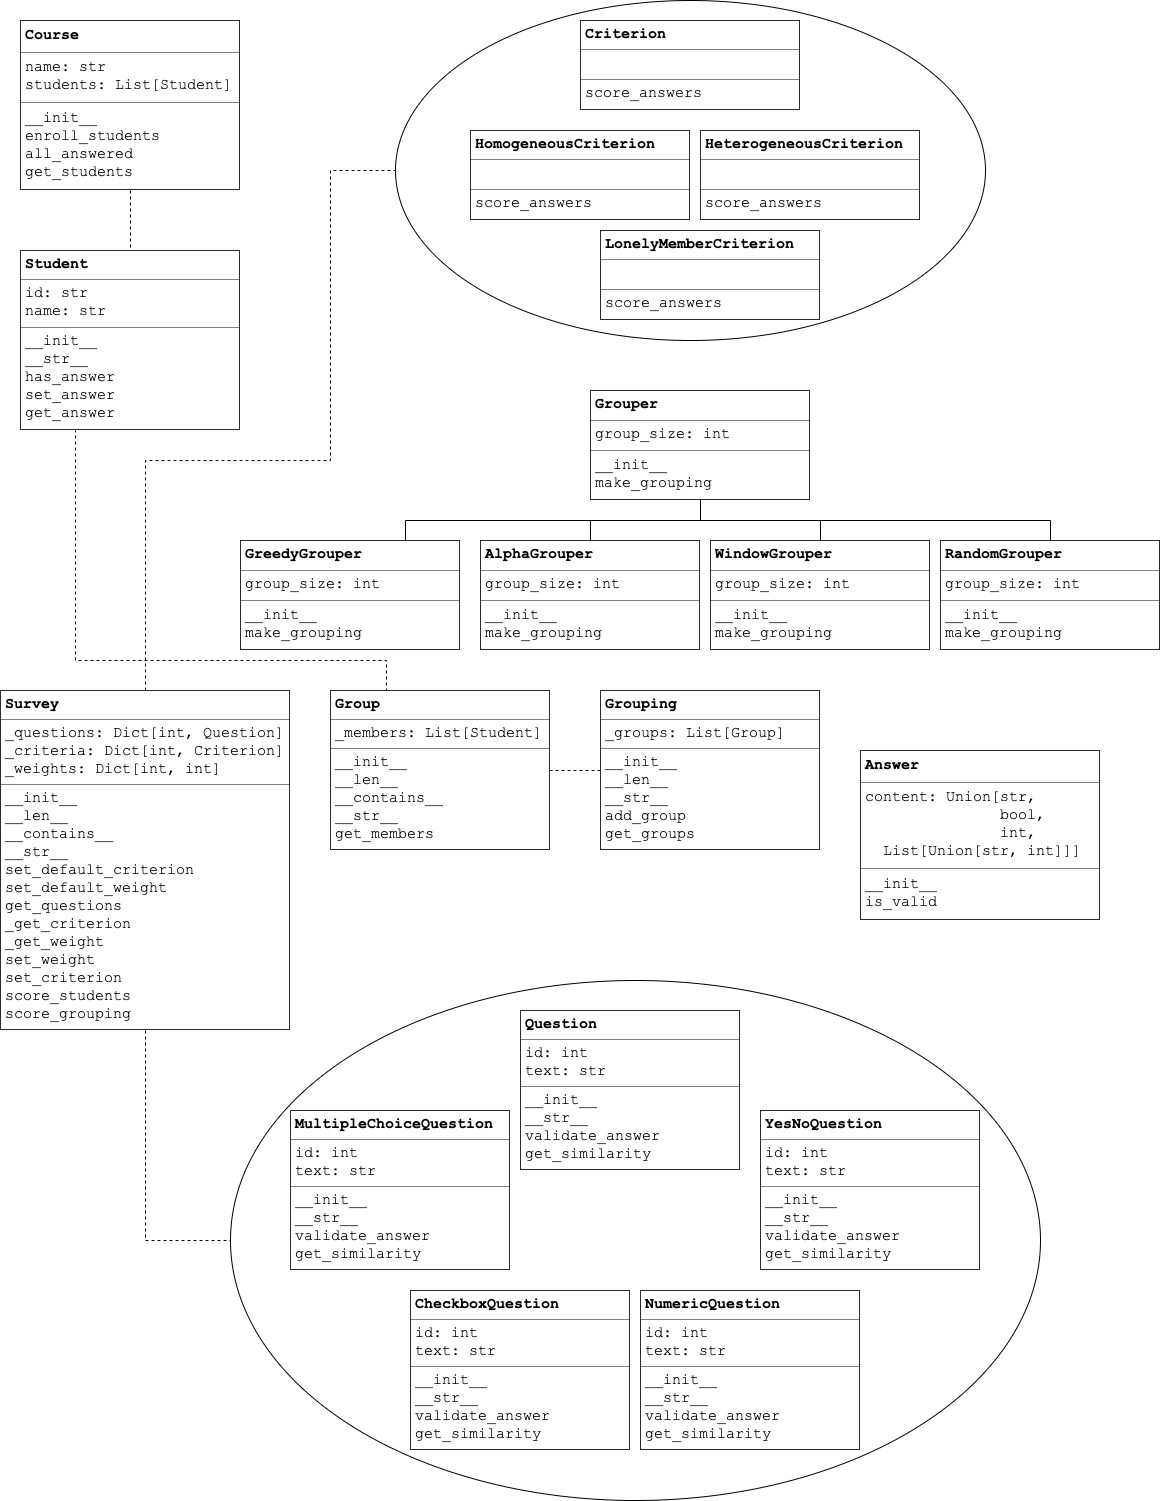
\includegraphics[width=0.8 \linewidth]{images/assignment_1/image_1.png}
\end{center}

\noindent Note that the attributes and methods shown in this diagram are only the ones
that we have given you in the starter code. You may need to define additional
private attributes or private helper methods.

\subsection*{Legend:}

\begin{itemize}
    \item dashed lines indicate a composition relationship between classes
    \item solid lines indicate an inheritance relationship between classes
    \item a solid circle around a group of classes indicates that there exists an inheritance relationship between these classes but it is not defined (you get to decide!)
\end{itemize}

\bigskip

\subsection*{Test your code!}

\begin{itemize}
    \item Try running the example\_tests.py file: all of the tests should fail because you haven’t written any code yet!
    \item Try running example\_usage.py file: you should get an error since you haven’t written any code yet!
    \item Open up the tests.py file: it is empty! This is where you will be writing all of your tests for this assignment
\end{itemize}

\subsection*{Something to think about!}
Unlike A0, you will be submitting code split across multiple files. Open up each
of the files and look at which functions and classes are defined in each file. Why do you think the files were organized
in this way? Is there a different way we could have organized these files?

\section*{2) Complete the Student Class}
The Student class represents a student who can be enrolled in a university
course.

\bigskip

\noindent The starter code for the \textit{Student} class can be found in \textit{course.py}. Open up this
file and read through the docstrings for each of the the \textit{Student} class’s methods.
Then, implement each of the methods in the \textit{Student} class.

\bigskip

\noindent Remember: you may need to define additional private attributes or
private helper methods!

\bigskip

\subsection*{Test your code!}
\begin{itemize}
    \item Write at least one unit test for each method in \textit{Student}. You are not
    required to write tests for initializers.
    \item You should write these tests in the \textit{tests.py} file.
    \item Once you have finished writing these tests, run all the tests in \textit{test.py}.
    Make sure your code passes all your tests before moving on.
    \item Run the tests in \textit{example\_tests.py}, the tests in the \textit{TestStudent} class should now pass.
\end{itemize}

\bigskip

\subsection*{Something to think about!}
The \textit{Student.has\_answer} method asks you to check if a student has a
valid answer to a given question. Do we have a way to determine if an answer is
valid or not yet? Answer: no and we won’t until we complete step 4. You may need
to come back and finish this method after completing step 5.

\section*{3) Complete the Course Class}
The \textit{Course} class represents a university course.

\bigskip

\noindent The starter code for the \textit{Course} class can be found in \textit{course.py}. Open up this
file and read through the docstrings for each of the the \textit{Course} class’s methods.
Then, implement each of the methods in the \textit{Course} class. You may find the
function \textit{sort\_students} helpful.

\bigskip

\noindent Remember: you may need to define additional private attributes or
private helper methods!

\subsection*{Test your code!}
\begin{itemize}
    \item Write at least one unit test for each method in \textit{Course}. You are not
    required to write tests for initializers.
    \item You should write these tests in the \textit{tests.py} file.
    \item Once you have finished writing these tests, run all the tests in
    \textit{test.py}. Make sure your code passes all your tests before moving on.
    \item Run the tests in \textit{example\_tests.py}, the tests in the \textit{TestCourse} class
    should now pass.
    \item Something to think about!
    \item The \textit{Course.all\_answered} method asks you to check if all students have
    a valid answer for every question in a \textit{Survey}. Which steps do you need to
    complete before you can finish this method? You may have to come back later to
    finish the \textit{Course.all\_answered} method.
\end{itemize}

\section*{4) Complete the Question Classes}
The file \textit{survey.py} contains an abstract \textit{Question} class, and the following classes
for representing different types of questions that you might find on a survey:

\begin{itemize}
    \item Question
    \item MultipleChoiceQuestion
    \item NumericQuestion
    \item YesNoQuestion
    \item CheckboxQuestion
\end{itemize}

\bigskip

\noindent As well as defining the text of the question itself, these classes also specify
what are valid answers to these questions.

\bigskip

\noindent Open up \textit{survey.py} and read through the docstrings for the methods in
these question classes.

\bigskip

You might notice that we have not defined any inheritance hierarchy between these
classes. You get to decide what it should be. However, in doing so you must follow
these rules:

\begin{enumerate}[1.]
    \item The abstract Question class should not inherit from any class other than
    object.
    \item All other \textit{Question} classes should inherit from the abstract
    \textit{Question} class either directly or indirectly.
    \item At least one non-abstract \textit{Question} class should inherit from another
    non-abstract Question class.
    \item There are many possible inheritance structures you could choose.
    Remember that one of the requirements for this assignment is to avoid
    writing duplicate code. Think about which sort of inheritance structure
    best lets you avoid duplicate code.
\end{enumerate}

\bigskip

\noindent Implement each of the methods in the Question classes. You may remove a method
that we included in the starter code for a child class if you wish to simply
inherit the parent’s method rather than to override it.

\noindent Remember: you may need to define additional private attributes or
private helper methods!

\subsection*{Test your code!}
\begin{itemize}
    \item Write at least one unit test for each method in each of the Question classes. You
    do not need to write tests for abstract methods or initializers but you do need
    to write tests for inherited methods.
    \item For example, even if you structure your code so that a child class inherits its
    \textit{validate\_answer} method without modification from the parent class, you still need
    to write separate tests for the \textit{validate\_answer} method in the parent
    class and the child class.
    \item You should write these tests in the \textit{tests.py} file.
    \item Once you have finished writing these tests, run all the tests in \textit{test.py}.
    Make sure your code passes all your tests before moving on.
    \item Run the tests in \textit{example\_tests.py}, the tests in the
    \textit{TestMultipleChoiceQuestion},\\ \textit{TestNumericQuestion},
    \textit{TestYesNoQuestion}, and \textit{TestCheckboxQuestion} class should now pass.
\end{itemize}

\subsection*{Something to think about!}
The \textit{validate\_answer} methods ask you to check if an answer is a valid answer for
this question. Do we have a enough information about the \textit{Answer} class
in order to complete this method now? You may need to come back and finish this
method after completing step 4.

\bigskip

\section*{5) Complete the Answer Class}
The \textit{Answer} class represents an answer to one of the questions you wrote
classes for in Step 3.

\bigskip

\noindent The starter code for the \textit{Answer} class can be found in \textit{survey.py}.
Open up this file and read through the docstrings for each of the the \textit{Answer}
class’s methods. Then, implement each of the methods in the \textit{Answer} class.

\bigskip

\noindent Remember: you may need to define additional private attributes or
private helper methods!

\bigskip

If you have not implemented the \textit{validate\_answer} methods in the \textit{Question}
classes, the \textit{Course.all\_answered} and the \textit{Student.has\_answer}
methods yet, go back and finish them now.

\bigskip

\subsection*{Test your code!}
\begin{itemize}
    \item Write at least one unit test for each method in \textit{Answer}. You are not required to write tests for initializers.
    \item You should write these tests in the \textit{tests.py} file.
    \item Once you have finished writing these tests, run all the tests in
    \textit{test.py}. Make sure your code passes all your tests before moving on.
    \item Run the tests in \textit{example\_tests.py}, the tests in the \textit{TestAnswer}
    class should now pass.
\end{itemize}

\subsection*{Something to think about!}
The \textit{Answer} class is one of the simplest classes that we will implement
in this assignment. What is the advantage of creating such a simple class? Are
there any disadvantages?

\section*{6) Complete the Criterion Class}
A criterion is a way of judging the quality of a group based on the group members’
answers to a particular question. For example, one criterion could be to want
groups with homogeneous answers to a question asking what year they are in.

\bigskip

\noindent The starter code defines several Criterion classes in \textit{criterion.py}. Open
up this file and read through the docstrings for each of the the \textit{Criterion}
class’ methods. The \textit{Criterion} classes are the classes in this file that
have “Criterion” in their name:

\begin{itemize}
    \item \textit{Criterion}
    \item \textit{HomogeneousCriterion}
    \item \textit{HeterogeneousCriterion}
    \item \textit{LonelyMemberCriterion}
\end{itemize}

\bigskip

You might notice that we have not defined any inheritance hierarchy between these
classes. You get to decide what it should be. However, in doing so you must
follow these rules:

\begin{enumerate}[1.]
    \item The abstract \textit{Criterion} class should not inherit from any class
    other than object.
    \item All other \textit{Criterion} classes should inherit from the abstract \textit{Criterion}
    class, either directly or indirectly.
    \item At least one non-abstract \textit{Criterion} class should inherit from another
    non-abstract Criterion class.
    \item There are many possible inheritanceses. You should NOT implement an
    initializer for these classes.
\end{enumerate}

\bigskip

\noindent Remember: You may remove a method defined in a child class if you wish to
simply inherit the parent’s method directly. structures you could choose. Remember
that one of the requirements for this assignment is to avoid writing duplicate code.
Think about which sort of inheritance structure best lets you avoid duplicate code.

\bigskip

\noindent Implement each of the methods in the \textit{Criterion} classes. You should NOT implement
an initializer for these classes.

\noindent Remember: you may need to define additional private helper methods!

\subsection*{Test your code!}
\begin{itemize}
    \item Write at least one unit test for each method in each of the \textit{Criterion}
    classes. You do not need to write tests for abstract methods but you do need to
    write tests for inherited methods.

    \item For example, even if you structure your code so that a child class
    inherits its \textit{score\_answers} method without modification from the parent class,
    you still need to write separate tests for the \textit{score\_answers} method in
    the parent class and the child class.

    \item You should write these tests in the \textit{tests.py} file.
    \item Once you have finished writing these tests, run all the tests in \textit{test.py}.
    Make sure your code passes all your tests before moving on.
    \item Run the tests in \textit{example\_tests.py}, the tests in the
    \textit{TestHomogeneousCriterion},\\ \textit{TestHeterogeneousCriterion}, and
    \textit{TestLonelyMemberCriterion} classes should now pass.
\end{itemize}

\subsection*{Something to think about!}
You are asked not to implement an initializer for the \textit{Criterion} classes.
Why is an initializer not necessary for these classes? If the \textit{Criterion}
classes do not define an initializer, will it be impossible to create instances
of these classes?

\section*{7) Complete the Group Class}
The \textit{Group} class represents a collection of one or more students.

The starter code for the \textit{Group} class can be found in \textit{grouper.py}.
Open up this file and read through the docstrings for each of the the \textit{Group}
class’s methods. Then implement each of the methods in the Group class.

\bigskip

\noindent Remember: you may need to define additional private attributes or
private helper methods!

\bigskip

\subsection*{Test your code!}
\begin{itemize}
    \item Write at least one unit test for each method in \textit{Group}. You are
    not required to write tests for initializers.
    \item You should write these tests in the \textit{tests.py} file.
    \item Once you have finished writing these tests, run all the tests in \textit{test.py}.
    Make sure your code passes all your tests before moving on.
    \item Run the tests in \textit{example\_tests.py}, the tests in the \textit{TestGroup}
    class should now pass.
    \item Something to think about!
\end{itemize}

\bigskip

\noindent You may find the Python \textit{set} type to be useful.

\bigskip

\noindent The \textit{Group.get\_members} method asks you to return a shallow
copy of the \textit{\_members} private attribute instead of simply returning the list that
\_members refers to. A \textit{shallow} copy of an object is a new object (with a different
\textit{id}) but whose contents are the same. For example,

\bigskip

\begin{lstlisting}[language=python,caption={worksheet\_17\_q1\_solution.py}]
    >>> dicts = [{1:2, 3:9}, {5:18}, {"adieu":7}]
    >>> copy = []
    >>> for item in dicts:
    ...     copy.append(item)
    ...
    >>> # dicts and copy are two different objects.
    >>> id(dicts)
    4485971264
    >>> id(copy)
    4485971200
    >>> # But each item in copy is an alias for an item in dicts.
    >>> For example:
    >>> id(dicts[2])
    4486046896
    >>> id(copy[2])
    4486046896
    >>> # With a Python list, any time we slice we get a new list.
    >>> # This provides an easy way to make a shallow copy.
    >>> another_copy = dicts[:]
    >>> id(another_copy)
    4485971008
    >>> id(another_copy[2])
    4486046896
\end{lstlisting}

\bigskip

\noindent In contrast, a \textbf{deep copy} has new objects at every level, so
it contains no aliases.

\bigskip

By returning a shallow copy, the \textit{Group.get\_members} method allows the client code
to mutate the individual Student objects but not the Group object itself. The same
reasoning holds for the \textit{Grouping.get\_groups} method in the next step.

\section*{8) Complete the Grouping Class}
The \textit{Grouping} class represents a collection of Group instances. An
instance of a \textit{Grouping} class can be used to represent every student in a course,
divided up into groups.

\bigskip

\noindent  The starter code for the Grouping class can be found in \textit{grouper.py}. Open
up this file and read through the docstrings for each of the the Grouping class’s
methods. Then, implement each of the methods in the \textit{Grouping} class.

\bigskip

\noindent Remember: you may need to define additional private attributes or
private helper methods!

\bigskip

\subsection*{Test your code!}

\begin{itemize}
    \item Write at least one unit test for each method in \textit{Grouping}. You
    are not required to write tests for initializers.
    \item You should write these tests in the tests.py file.
    \item Once you have finished writing these tests, run all the tests in test.py. Make sure your code passes all your tests before moving on.
    \item Run the tests in \textit{example\_tests.py}, the tests in the \textit{TestGrouping} class
    should now pass.
\end{itemize}

\bigskip

\subsection*{Something to think about!}
An instance of the \textit{Grouping} class starts out containing zero groups and
more can be added later using the \textit{Grouping.add\_group}. On the other
hand, an instance of the \textit{Group} class starts out with some members and more cannot
be added later. Why might we have chosen to implement these classes differently?
What does this design choice tell us about how these classes are intended to be used?

\section*{9) Complete the Survey Class}

\section*{10) Complete the helper functions in \textit{grouper.py}}

\section*{11) Complete the Grouper Classes}

\section*{12) Test the Code Again}

\section*{13) Submit your work}

\end{document}